%% LyX 2.3.2-2 created this file.  For more info, see http://www.lyx.org/.
%% Do not edit unless you really know what you are doing.
\documentclass[english]{article}
\usepackage[T1]{fontenc}
\usepackage[latin9]{luainputenc}
\usepackage{geometry}
\geometry{verbose,tmargin=2cm,bmargin=2cm,lmargin=2cm,rmargin=2cm,headheight=2cm,headsep=2cm,footskip=2cm}
\usepackage{float}
\usepackage{amsmath}
\usepackage{amssymb}
\usepackage{cancel}
\usepackage{stackrel}
\usepackage{graphicx}

\makeatletter
\@ifundefined{showcaptionsetup}{}{%
 \PassOptionsToPackage{caption=false}{subfig}}
\usepackage{subfig}
\makeatother

\usepackage{babel}
\begin{document}

\section{Ejercicio 1}

\subsection{Ejercicio 2b de la guia de sistemas discretos}

Se pide hallar la ecuacion en diferencias el siguiente diagrama de
bloques:
\begin{center}
\begin{figure}[H]

\begin{centering}
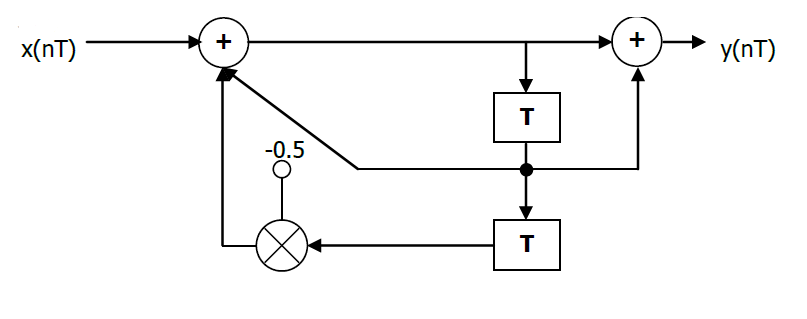
\includegraphics[scale=0.3]{Imagenes/DiagramaDelEj2b.PNG}
\par\end{centering}
\caption{Diagrama en bloques del sistema del Ej:2b}

\end{figure}
\par\end{center}

Asumiendo que el sistema esta relajado y que la entrada es causal,
lo que quiere decir que:

$\begin{cases}
y(nT)=x(nT)=0; & \forall n<0\end{cases}$

Se tiene el siguiente diagrama en boques luego de aplicarle la transformada
Z a la red:
\begin{center}
\begin{figure}[H]

\caption{Diagram de bloques del sistema en Z}

\end{figure}
\par\end{center}

\subsection{Ejercicio 9 de la guia de sistemas discretos}

Se pide determinar la respuesta al impulso, al escalon y la respuesta
en frecuencia del siguiente sistema de segundo orden:
\begin{center}
\begin{figure}[H]
\begin{centering}
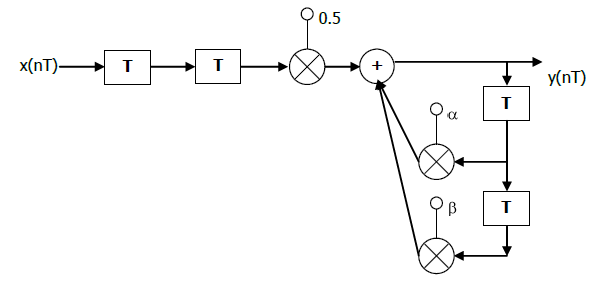
\includegraphics[scale=0.3]{Imagenes/DiagramaEj9.PNG}
\par\end{centering}
\caption{Sistema del ej9 de sistemas discretos}

\end{figure}
\par\end{center}

Los valores de $\alpha$ y $\beta$ son:

a) $\alpha=1$, $\beta=-\frac{1}{2}$

b) $\alpha=\frac{1}{2}$, $\beta=-\frac{1}{8}$

c) $\alpha=\frac{5}{4}$, $\beta=-\frac{25}{32}$

De dicha red se obtiene la siguiente ecuacion en diferencias:
\begin{center}
\begin{equation}
\frac{1}{2}x(nT-2T)+\alpha y(nT-T)+\beta y(nT-2T)=y(nT)\label{eq:1}
\end{equation}
\par\end{center}

Para simplificar las cuentas, se normaliza el per�odo a la unidad
($T=1$) y luego se desnormaliza cuando se llega a los resultados:
\begin{center}
$\frac{1}{2}x(n-2)+\alpha y(n-1)+\beta y(n-2)=y(n)$
\par\end{center}

Aplicando la transformada Z a la ecuacion (\ref{eq:1})se obtiene
la siguiente expresion:
\begin{center}
$\frac{1}{2}z^{-2}[z^{2}.x(-2)+z.x(-1)+X(z)]+\alpha.z^{-1}[z.y(-1)+Y(z)]+\beta.z^{-2}[z^{2}y(-2)+z.y(-1)+Y(z)]=Y(z)$
\par\end{center}

Donde $X(z)$ e $Y(z)$ son las transformadas Z de $x(n)$ e $y(n)$
respectivamente.

Considerando al sistema relajado(condiciones iniciales nulas) y la
entrada como causal la ecuacion anterior se simplifica a:
\begin{center}
$\frac{1}{2}z^{-2}X(z)+\alpha z^{-1}Y(z)+\beta z^{-2}Y(z)=Y(z)$
\par\end{center}

\begin{center}
$\frac{1}{2}z^{-2}X(z)=Y(z)[1-\beta z^{-2}-\alpha z^{-1}]$
\par\end{center}

\begin{center}
\begin{equation}
\frac{Y(z)}{X(z)}=H(z)=\frac{z^{2}}{z^{2}}.\frac{\frac{1}{2}z^{-2}}{1-\beta z^{-2}-\alpha z^{-1}}=\frac{1}{2}.\frac{1}{z^{2}-\alpha z-\beta}\label{eq:2}
\end{equation}
\par\end{center}

Los polos de $H(z)$(transformada Z de la respuesta impulsiva) tienen
la siguiente forma:
\begin{center}
$\frac{\alpha\pm\sqrt{\alpha^{2}+4\beta}}{2}=\frac{\alpha}{2}\pm\sqrt{(\frac{\alpha}{2})^{2}+\beta}$
\par\end{center}

Tanto para el caso a), b) y c) los valores de $\alpha$ y $\beta$
son tales que cumplen que:
\begin{center}
$(\frac{\alpha}{2})^{2}+\beta<0\Longrightarrow z_{1,2}=\frac{\alpha}{2}\pm j\sqrt{-[(\frac{\alpha}{2})^{2}+\beta]}$
\par\end{center}

Por conveniencia definimos $\omega=\sqrt{-[(\frac{\alpha}{2})^{2}+\beta]}$

Se puede reescribir $H(z)$ como:
\begin{center}
$H(z)=\frac{1}{2}.\frac{1}{(z-z_{1})(z-z_{2})}$
\par\end{center}

Una forma posible de obtener la antitransformada de $H(z)$ es medinte
residuos utilizando la siguiente formula:
\begin{center}
$h(n)=u(n).\sum_{i=1}^{M}Res\{H(z).z^{n-1},z_{i}\}$
\par\end{center}

En este caso las singularidades de $H(z).z^{n-1}$ son:
\begin{center}
$z_{1,2}=\frac{\alpha}{2}\pm j\omega$ y para n=0$z_{3}=0$
\par\end{center}

Los residuos correspondientes son:
\begin{itemize}
\item $lim_{z\rightarrow z_{1}}\cancel{(z-z_{1})}.\frac{1}{2}\frac{z^{n-1}}{\cancel{(z-z_{1})}(z-z_{2})}=\frac{1}{2}.\frac{[(\frac{\alpha}{2})+j\omega]^{n-1}}{2j\omega}\stackrel{Polares}{=}\frac{1}{j4\omega}.(\sqrt{-\beta})^{n-1}e^{j(n-1)\theta}$
\item $lim_{z\rightarrow z_{2}}\cancel{(z-z_{2})}.\frac{1}{2}\frac{z^{n-1}}{(z-z_{1})\cancel{(z-z_{2})}}=-\frac{1}{2}.\frac{[(\frac{\alpha}{2})-j\omega]^{n-1}}{2j\omega}\stackrel{Polares}{=}-\frac{1}{j4\omega}.(\sqrt{-\beta})^{n-1}e^{-j(n-1)\theta}$
\item $lim_{z\rightarrow0}\cancel{(z)}.\frac{1}{2}.\frac{1}{\cancel{z}(z-z_{1})(z-z_{2})}=\frac{1}{2}.\frac{1}{z_{1}.z_{2}}=\frac{1}{2}.\frac{1}{z_{1}.\bar{z_{1}}}=\frac{1}{2}.\frac{1}{|z_{1}|^{2}}=\frac{1}{2}.\frac{1}{(\frac{\alpha}{2})^{2}-(\frac{\alpha}{2})^{2}-\beta}=-\frac{1}{2}.\frac{1}{\beta}$

Donde $\theta=arctg(\frac{2\omega}{\alpha})$
\end{itemize}
De dichos residuos se obtiene como expresion de antitransformada:
\begin{center}
$h(n)=-\frac{1}{2}.\frac{1}{\beta}\delta(n)+u(n)[\frac{1}{j4\omega}.(\sqrt{-\beta})^{n-1}e^{j(n-1)\theta}-\frac{1}{j4\omega}.(\sqrt{-\beta})^{n-1}e^{-j(n-1)\theta}]$
\par\end{center}

\begin{center}
$h(n)=\frac{1}{2}[-\frac{1}{\beta}\delta(n)+u(n).\frac{(\sqrt{-\beta})^{n-1}}{\omega}.\underset{\overbrace{sin[(n-1)\theta]}}{(\frac{e^{j(n-1)\theta}-e^{-j(n-1)\theta}}{2j})}]$
\par\end{center}

Si evaluamos en n=0 se obtiene que:
\begin{center}
$h(0)=\frac{1}{2}[-\frac{1}{\beta}+\frac{1}{\omega.\sqrt{-\beta}}.sin(-\theta)]=\frac{1}{2}[-\frac{1}{\beta}-\frac{1}{\cancel{\omega}\sqrt{-\beta}}.\frac{\cancel{\omega}}{\sqrt{-\beta}}]=\frac{1}{2}[-\frac{1}{\beta}+\frac{1}{\beta}]=0$
\par\end{center}

Por lo que se puede reescribir la respuesta impulsiva del sistema
como:
\begin{center}
$h(n)=\frac{1}{2\omega}.(\sqrt{-\beta})^{n-1}sin[(n-1)\theta].u(n-1)$
\par\end{center}

Luego, teniendo en cuenta el per�odo de muestreo T, se reescribe se
llega a la forma final de la respuesta como:
\begin{center}
\begin{equation}
h(nT)=\frac{1}{2\omega}.(\sqrt{-\beta})^{nT-T}sin[(nT-T)\theta].u(nT-T)\label{eq:3}
\end{equation}
\par\end{center}

Se realizo un script(``Ej9-impulso'') para graficar esta respuesta
impulsiva para los tres casos a), b) y c), el resultado fue el siguiente:
\begin{center}
\begin{figure}[H]
\begin{raggedright}
\subfloat[Item a( $\alpha=1$, $\beta=-\frac{1}{2}$)]{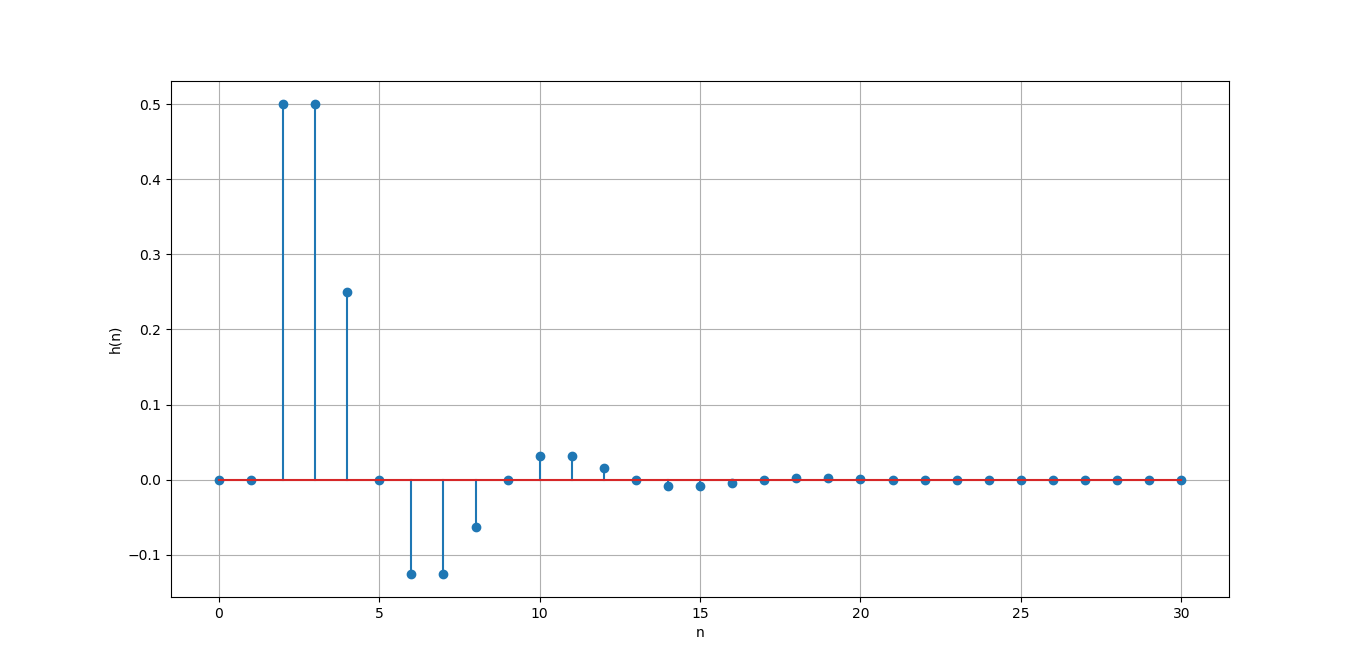
\includegraphics[scale=0.2]{Imagenes/Ej9-ItemA}

}\subfloat[Item b( $\alpha=\frac{1}{2}$, $\beta=-\frac{1}{8}$)]{\begin{raggedright}
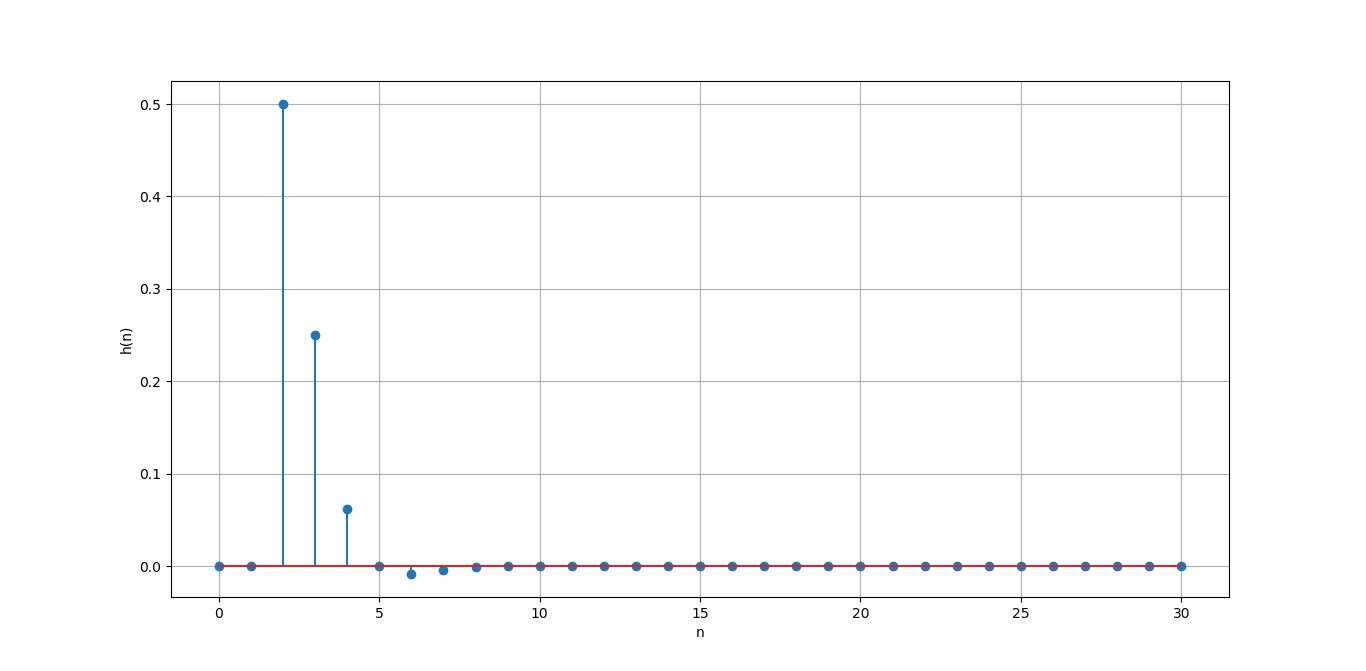
\includegraphics[scale=0.2]{Imagenes/Ej9-ItemB}
\par\end{raggedright}

}
\par\end{raggedright}
\begin{centering}
\subfloat[Item c( $\alpha=\frac{5}{4}$, $\beta=-\frac{25}{32}$)]{\begin{centering}
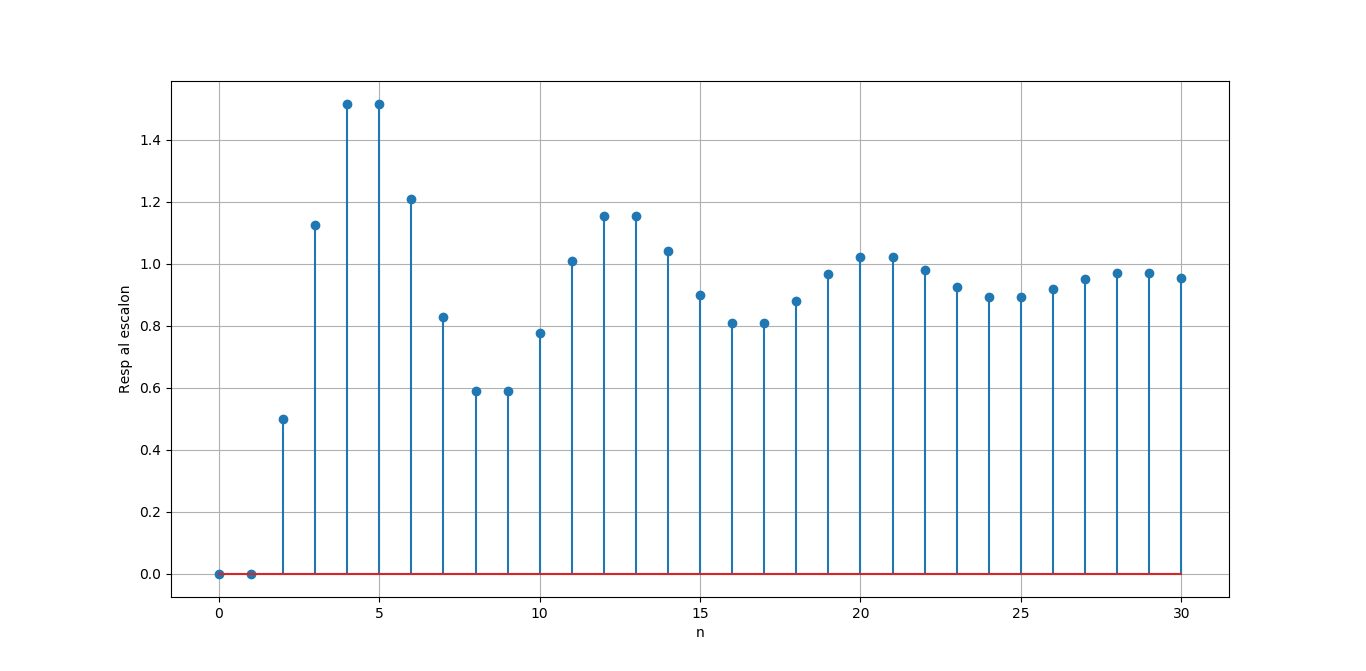
\includegraphics[scale=0.2]{Imagenes/Ej9-Escalon-ItemC}
\par\end{centering}
}
\par\end{centering}
\caption{Graficas de las respuestas impulsivas}

\end{figure}
\par\end{center}

\subsubsection{Respuesta al escalon}

Para la respuesta al escalon del sistema se comenzo planteando la
forma generica de la respuesta de un sistema LTI en tiempo discreto:
\begin{center}
$y(n)=(h*u)(n)$
\par\end{center}

Transformando ambos lados de la ecuacion se obtiene:
\begin{center}
$Y(z)=H(z).Z\{u(n)\}(z)$
\par\end{center}

Donde:
\begin{center}
$Z\{u(n)\}(z)=\sum_{k=0}^{+\infty}z^{-k}=\frac{1}{1-z^{-1}}=\frac{z}{z-1},|z|>1$
\par\end{center}

Entonces reemplazando la tranformada del escalon calculada previamente
y $H(z)$ por lo obtenido en (\ref{eq:2}), se tiene:
\begin{center}
$Y(z)=\frac{1}{2}.\frac{z}{(z-1)(z^{2}-\alpha z-\beta)}$
\par\end{center}

Decomponiendo en fracciones simples:
\begin{center}
$Y(z)=\frac{A}{z-1}+\frac{Bz+C}{z^{2}-\alpha z-\beta}\Rightarrow\frac{z}{2}=A(z^{2}-\alpha z-\beta)+B.z(z-1)+C(z-1)$
\par\end{center}

$\underline{z=1}$
\begin{center}
$\frac{1}{2}=A(1-\alpha-\beta)\rightarrow A=\frac{1}{2(1-\alpha-\beta)}$
\par\end{center}

$\underline{z=0}$
\begin{center}
$0=-\frac{\beta}{2(1-\alpha-\beta)}-C\rightarrow C=-\frac{\beta}{2(1-\alpha-\beta)}$
\par\end{center}

$\underline{z=-1}$
\begin{center}
$-\frac{1}{2}=\frac{1+\alpha-\beta}{2(1-\alpha-\beta)}+2B+\frac{\cancel{2}\beta}{\cancel{2}(1-\alpha-\beta)}$
\par\end{center}

\begin{center}
$-\frac{1}{2}-\frac{1+\alpha-\beta}{2(1-\alpha-\beta)}-\frac{\cancel{2}\beta}{\cancel{2}(1-\alpha-\beta)}=2B$
\par\end{center}

\begin{center}
$\frac{-1+\cancel{\alpha}+\cancel{\beta}-1-\cancel{\alpha}+\cancel{\beta}-\cancel{2\beta}}{2(1-\alpha-\beta)}=2B\rightarrow B=-\frac{1}{2(1-\alpha-\beta)}$
\par\end{center}

Teniendo en cuenta que:
\begin{itemize}
\item $Z\{\delta(n-k)\}=z^{k}$
\item $\delta(n-k)*x(n)=x(n-k)$
\end{itemize}
La antitransformada de $Y(z)$ es:
\begin{center}
$y(n)=A.u(n-1)+2C.h(n)+2B.h(n-1)$
\par\end{center}

\begin{center}
\begin{equation}
y(n)=\frac{1}{2(1-\alpha-\beta)}u(n-1)-\frac{\beta}{1-\alpha-\beta}h(n)-\frac{1}{1-\alpha-\beta}h(n+1)
\end{equation}
\par\end{center}

Al igual que para le respuesta impulsiva se realizo un script(``Ej9-escalon'')
para graficar la repuesta al escalon de cada item.
\begin{center}
\begin{figure}[H]
\begin{centering}
\subfloat[Item A( $\alpha=1$, $\beta=-\frac{1}{2}$)]{\begin{centering}
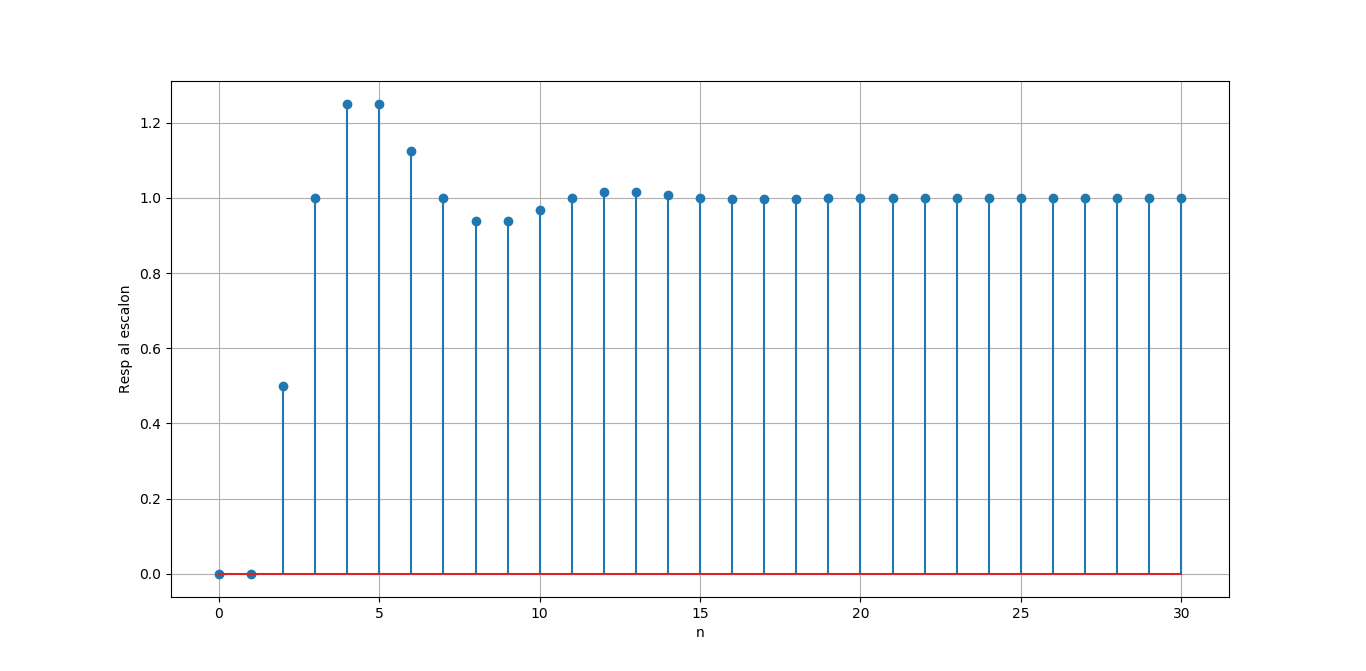
\includegraphics[scale=0.25]{Imagenes/Ej9-Escalon-ItemA}
\par\end{centering}

}\subfloat[Item b( $\alpha=\frac{1}{2}$, $\beta=-\frac{1}{8}$)]{
\begin{centering}
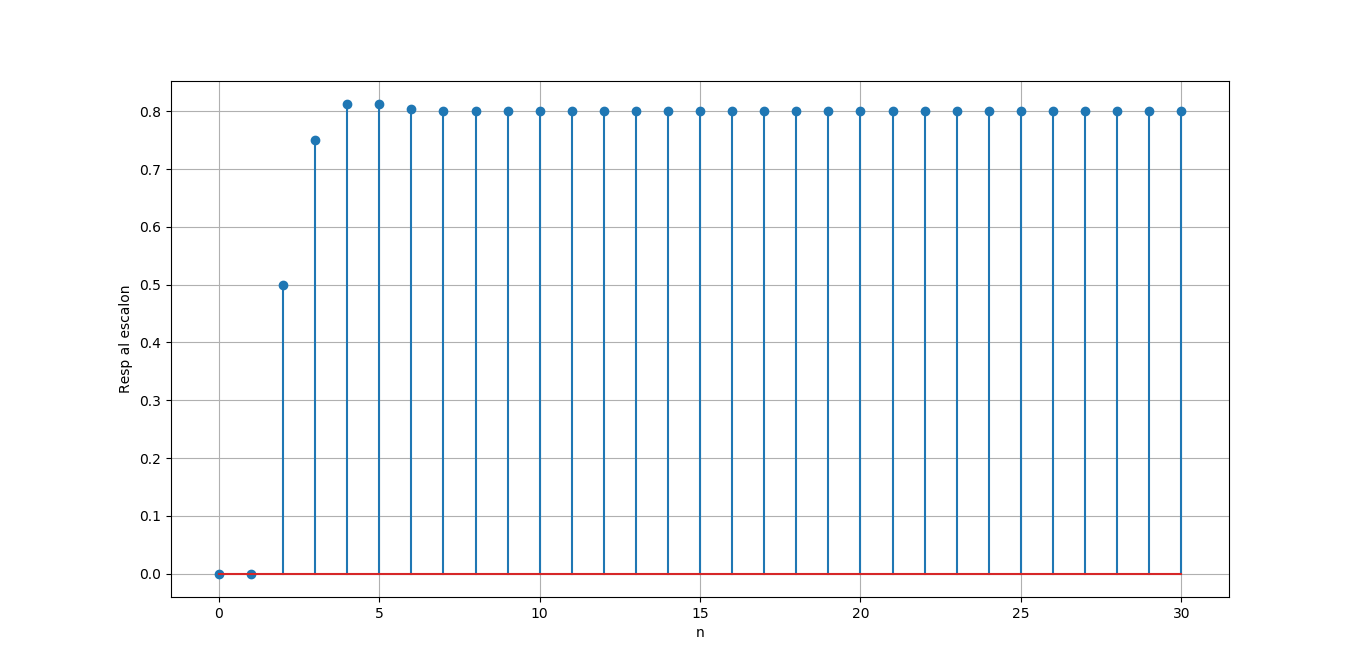
\includegraphics[scale=0.2]{Imagenes/Ej9-Escalon-ItemB}
\par\end{centering}
}
\par\end{centering}
\begin{centering}
\subfloat[Item c]{\begin{centering}
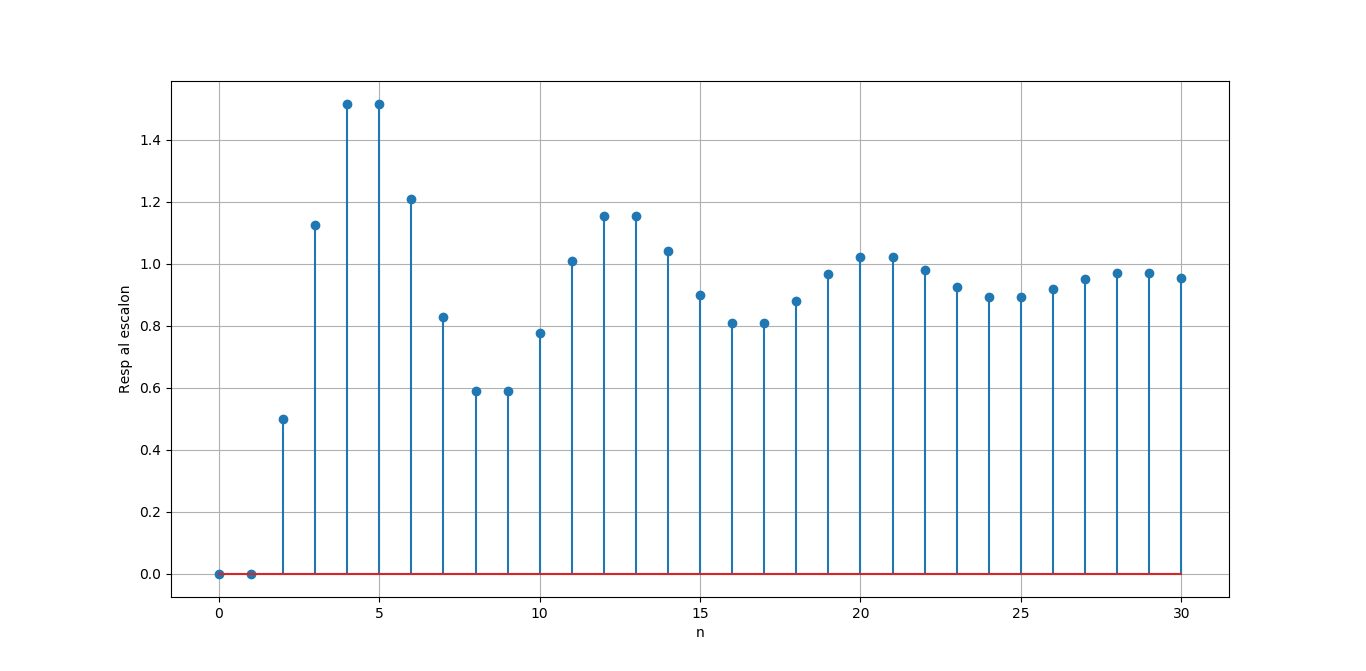
\includegraphics[scale=0.25]{Imagenes/Ej9-Escalon-ItemC}
\par\end{centering}

}
\par\end{centering}
\caption{Graficas de la respuesta al escalon}

\end{figure}
\par\end{center}

\section{Ejercicio 3.a}

Se pide verificar la estabilidad del siguiente filtro recursivo:
\begin{center}
\begin{equation}
H(z)=\frac{z^{6}}{6z^{6}+5z^{5}+4z^{4}+3z^{3}+2z^{2}+z+1}
\end{equation}
\par\end{center}

Asumiendo que el sistema es causal se tiene que el sistema es estable
si se tiene que todas sus singularidades estan dentro del circulo
untario($|z|<1$).

Se deinfe como funcion caracteristica del sistema a:
\begin{center}
$f(z)=6z^{6}+5z^{5}+4z^{4}+3z^{3}+2z^{2}+z+1=0$
\par\end{center}

\begin{center}
\begin{equation}
f(z)=z^{6}+\frac{5}{6}z^{5}+\frac{2}{3}z^{4}+\frac{1}{2}z^{3}+\frac{1}{3}z^{2}+\frac{1}{6}z+\frac{1}{6}=0\label{eq:6}
\end{equation}
\par\end{center}

Para que el sistemaa sea estable debe cumplir:
\begin{enumerate}
\item Todos los coeficientes de (\ref{eq:6}) deben ser menor al orden de
la misma
\item $|\frac{a_{0}}{a_{n}}|<1$, donde $a_{0}$ es el coeficiente que acompana
al ttermino independiente y $a_{n}$ el que acompana a $z^{n}$
\end{enumerate}
Una simple inspeccion de la f(z) muestra que se cumple la condicion
1, en cuanto a la condicion 2 $|\frac{a_{0}}{a_{n}}|=\frac{1}{6}<1$.
Esto significa que en primera instancia la funcion caracteristica
cumple con las condiciones necesarias.

Como siguiente paso se arman las matrices triangulares correspondientes:
\begin{center}
$H_{1}=\left(\begin{array}{ccccccc}
6 & 5 & 4 & 3 & 2 & 1 & 1\\
0 & 6 & 5 & 4 & 3 & 2 & 1\\
0 & 0 & 6 & 5 & 4 & 3 & 2\\
0 & 0 & 0 & 6 & 5 & 4 & 3\\
0 & 0 & 0 & 0 & 6 & 5 & 4\\
0 & 0 & 0 & 0 & 0 & 6 & 5\\
0 & 0 & 0 & 0 & 0 & 0 & 6
\end{array}\right)$, $H_{2}=\left(\begin{array}{ccccccc}
6 & 5 & 4 & 3 & 2 & 1 & 1\\
5 & 4 & 3 & 2 & 1 & 1 & 0\\
4 & 3 & 2 & 1 & 1 & 0 & 0\\
3 & 2 & 1 & 1 & 0 & 0 & 0\\
2 & 1 & 1 & 0 & 0 & 0 & 0\\
1 & 1 & 0 & 0 & 0 & 0 & 0\\
1 & 0 & 0 & 0 & 0 & 0 & 0
\end{array}\right)$
\par\end{center}

De la suma de ambas matrices se obtiene:
\begin{center}
$H_{7}=H_{1}+H_{2}=\left(\begin{array}{ccccccc}
12 & 10 & 8 & 6 & 4 & 2 & 2\\
5 & 10 & 8 & 6 & 4 & 3 & 1\\
4 & 3 & 8 & 6 & 5 & 3 & 2\\
3 & 2 & 1 & 7 & 5 & 4 & 3\\
2 & 1 & 1 & 0 & 6 & 5 & 4\\
1 & 1 & 0 & 0 & 0 & 6 & 5\\
1 & 0 & 0 & 0 & 0 & 0 & 6
\end{array}\right)$
\par\end{center}

Definiendo los ddeterminantes internos de la matriz como:
\begin{itemize}
\item $\nabla_{1}=7>0$
\item $\nabla_{3}=\left|\begin{array}{ccc}
8 & 6 & 5\\
1 & 7 & 5\\
1 & 0 & 6
\end{array}\right|=295>0$
\item $\nabla_{5}=\left|\begin{array}{ccccc}
10 & 8 & 6 & 4 & 3\\
3 & 8 & 6 & 5 & 3\\
2 & 1 & 7 & 5 & 4\\
1 & 1 & 0 & 6 & 5\\
1 & 0 & 0 & 0 & 6
\end{array}\right|=12383>0$
\item $\nabla_{7}=\left|\begin{array}{ccccccc}
12 & 10 & 8 & 6 & 4 & 2 & 2\\
5 & 10 & 8 & 6 & 4 & 3 & 1\\
4 & 3 & 8 & 6 & 5 & 3 & 2\\
3 & 2 & 1 & 7 & 5 & 4 & 3\\
2 & 1 & 1 & 0 & 6 & 5 & 4\\
1 & 1 & 0 & 0 & 0 & 6 & 5\\
1 & 0 & 0 & 0 & 0 & 0 & 6
\end{array}\right|=507408>0$
\end{itemize}
El calculo de los determinantes internos de la matriz se realizo con
el script de python titulado ``Determinantes''.

Como la funcion caracteristica del sistema cumple las condiciones
necesarias mencionadas previamente y todos sus determinantes internos
son positivos, se concluye que el sistema es estable.

\section{Ejercicio 6}

\subsection{Item a}

Se pide demostrar la siguiente igualdad:
\begin{center}
$|H(e^{j\omega})|^{2}=H(z).H(z^{-1})|_{z=e^{j\omega}}$
\par\end{center}

demostracion:
\begin{center}
$H(z).H(z^{-1})\stackrel{definicion}{=}(\stackrel[k=-\infty]{k=+\infty}{\sum}h(k).z^{-k}).(\stackrel[n=-\infty]{n=+\infty}{\sum}h(n).z^{n})$
\par\end{center}

\begin{center}
$\overset{distributiva}{=}\stackrel[k=-\infty]{k=+\infty}{\sum}(\stackrel[n=-\infty]{n=+\infty}{\sum}h(n).z^{n})h(k).z^{-k}\stackrel{z=e^{j\omega}}{\rightarrow}\stackrel[k=-\infty]{k=+\infty}{\sum}(\stackrel[n=-\infty]{n=+\infty}{\sum}h(n).e^{jn\omega})h(k).e^{-jk\omega}$
\par\end{center}

\begin{center}
$\stackrel{Conjugado}{=}\stackrel[k=-\infty]{k=+\infty}{\sum}\overline{(\stackrel[n=-\infty]{n=+\infty}{\sum}\overline{h(n)}.e^{-jn\omega})}h(k).e^{-jk\omega}\stackrel{h\epsilon\mathbb{R}}{=}\stackrel[k=-\infty]{k=+\infty}{\sum}\overline{(\stackrel[n=-\infty]{n=+\infty}{\sum}h(n).e^{-jn\omega})}h(k).e^{-jk\omega}$
\par\end{center}

\begin{center}
$\stackrel{definicion}{=}\stackrel[k=-\infty]{k=+\infty}{\sum}\overline{H(\omega)}h(k).e^{-jk\omega}=\overline{H(\omega)}.\stackrel[k=-\infty]{k=+\infty}{\sum}h(k).e^{-jk\omega}\stackrel{definicion}{=}\overline{H(\omega)}.H(\omega)=|H(\omega)|^{2}$
\par\end{center}

\subsection{Item b}

Se pide demostrar que el siguiente sistema es un filtro pasa todo(ganancia
unitaria para toda frecuencia):
\begin{center}
$H(z)=\frac{1-az+bz^{2}}{b-az+z^{2}}$
\par\end{center}

demostracion:
\begin{center}
$|H(e^{j\omega})|^{2}=H(z).H(z^{-1})=\frac{(1-az+bz^{2})}{b-az+z^{2}}.\frac{(1-az^{-1}+bz^{-2})}{b-az^{-1}+z^{-2}}$
\par\end{center}

\begin{center}
$=\frac{\cancel{bz^{2}-(ab+a)z+1+a^{2}+b^{2}-(ab+a)z^{-1}+bz^{-2}}}{\cancel{bz^{2}-(ab+a)z+1+a^{2}+b^{2}-(ab+a)z^{-1}+bz^{-2}}}.1=1$
\par\end{center}

\subsection{Item c}
\end{document}
